\documentclass{article}
\usepackage[utf8]{inputenc}
\usepackage{blindtext}
\usepackage[a4paper, margin=0.5in]{geometry}
\usepackage{graphicx}
\usepackage[T1]{fontenc}
\usepackage{url}
\usepackage{float}
\usepackage{titlesec}

\setcounter{secnumdepth}{4}



\begin{document}


\title{Physics Research Internship Report}
\author{Samsam Lee}

\date{September 2022}


%\maketitle


\begin{center}
    \Large
    \textbf{Physics Research Internship Report}
        
    \vspace{0.4cm}
    \large
    September 2022
        
    \vspace{0.4cm}
    \textbf{Samsam Lee}
       
    \vspace{0.9cm}
    \textbf{Imperial College London ECTS Report}
\end{center}

\section{Introduction}

This physics summer research internship project is lead by Professor Ong at The Chinese University Of Hong Kong. The project is primarily on Michelson Interferometer and stabilisation of light intensity using PID algorithm, which is followed by Interference Lithography using the previous set-up.


\section{Michelson Interferometer}

Before starting the PID project, we (me and my lab partner) learnt the theory of interference and built a Michelson interferometer. SMC100 motor and DAQ with a photoresistor detector is used with lab view to plot a spectrum:

\begin{figure}[H]
\centering
\includegraphics[width=0.3\textwidth,angle=0,origin=c]{pictures/IMG_4EC45EC59B99-1.jpeg}
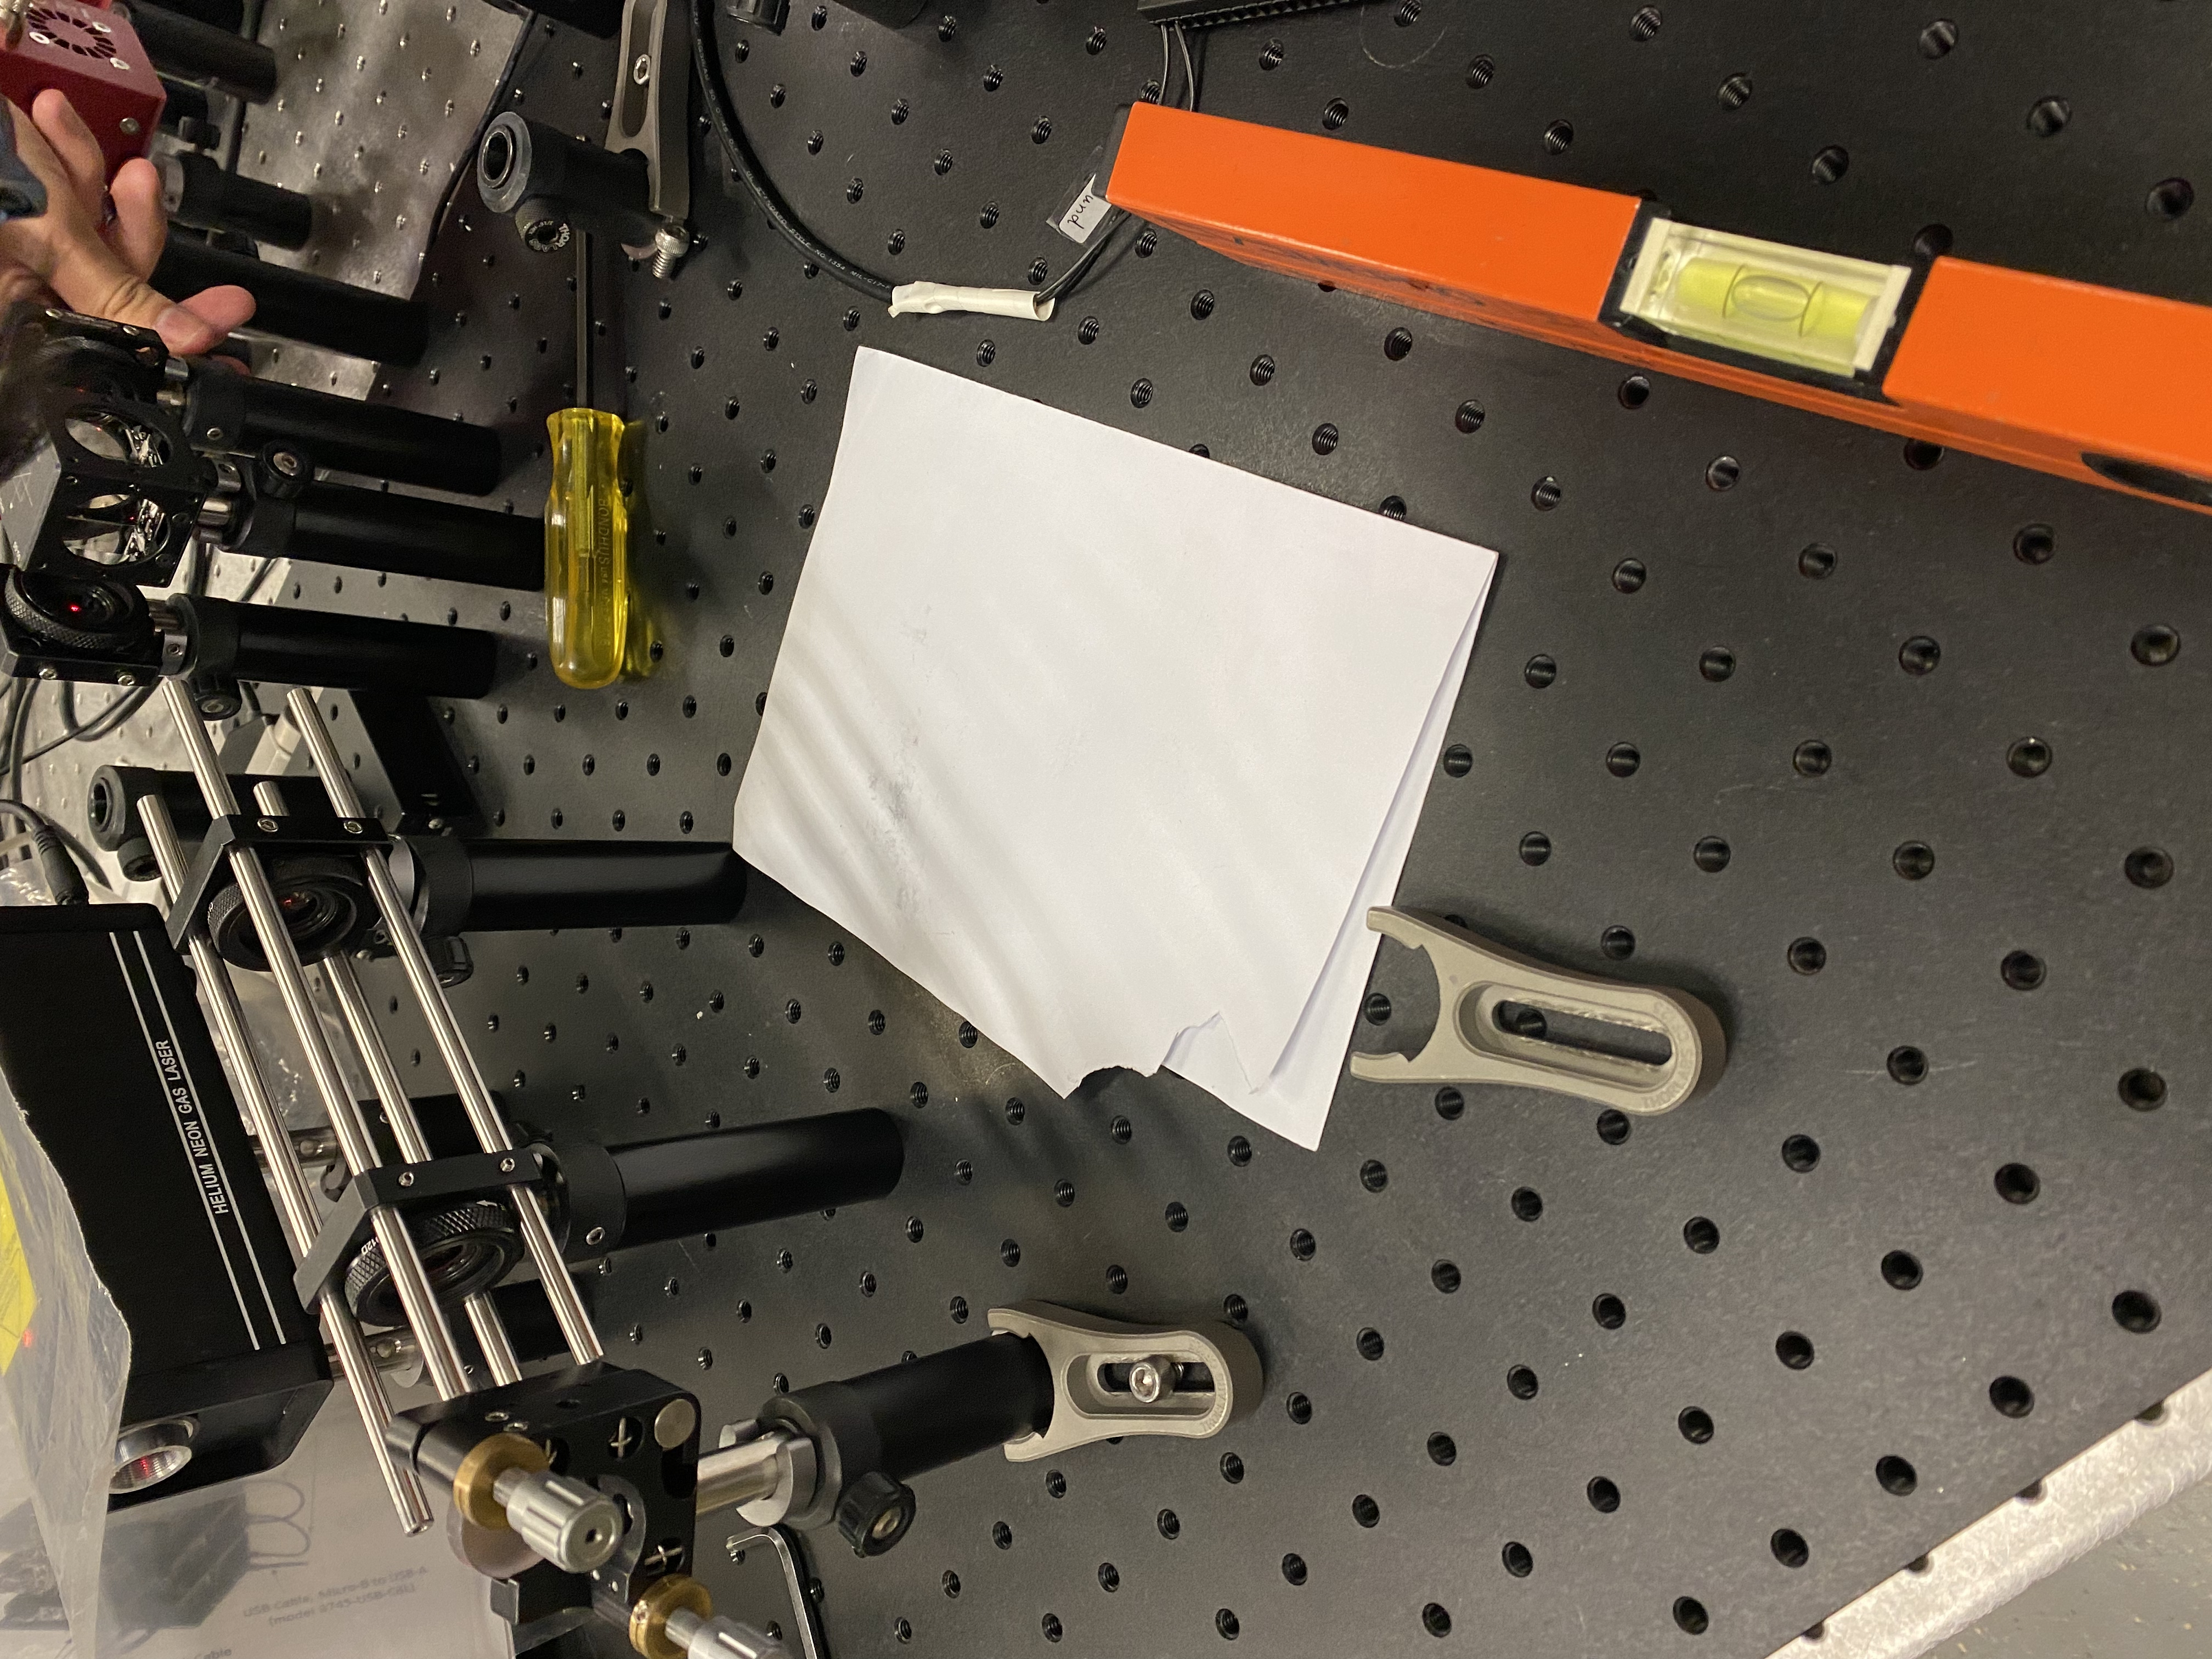
\includegraphics[width=0.4\textwidth,angle=-90,origin=c]{pictures/IMG_0864.jpg}
\end{figure}


\section{PID algorithm}
The aim for PID is to minimise the light intensity fluctuation to properly perform interference lithography (discussed in the later section). We use a similar set-up as Michelson interferometer in the interference lithography. 

Due to the lack of experience and knowledge in this field, I begin doing research on related fields, ie, maths behind PID and use of labview. Then we proceed to build a simple experiment set up for learning purpose:\\


\begin{figure}[H]
\centering
\includegraphics[width=0.4\textwidth,angle=0,origin=c]{pictures/IMG_B17822D656A3-1.jpeg}
\end{figure}


\textbf{Aim:}

Find the maximum possible detected intensity and lock the intensity (stabilise it at that point) \\


We performed the experiment using labview.
The code logic is as follows:\\

\begin{figure}[H]
\centering
\includegraphics[width=0.4\textwidth,angle=0,origin=c]{pictures/IMG_3248C6367539-1.jpeg}
\end{figure}

\subsection{Using Python as an alternative of labview}

As using script based programming languages (ie, c++ or python) are more convenient while performing experiments with more complex programming logic, I developed a python controller library for the SMC100 motor. Details and the codes are posted on another page.


\subsection{Using PID to stabilise the intensity in interference:}

We proceeded to the main part of the PID project, which is to stabilise  the intensity using PID. The set up is basically the same as the one in Michelson interferometer, but instead of driving the motor along the trail indefinitely to plot an intensity-time graph, we drive the motor using the PID algorithm so that the motor moves forward and backward according to the intensity change.


Intensity response when we slap on the table to change the intensity. The intensity goes back to the setpoint. 

\begin{figure}[H]
\centering
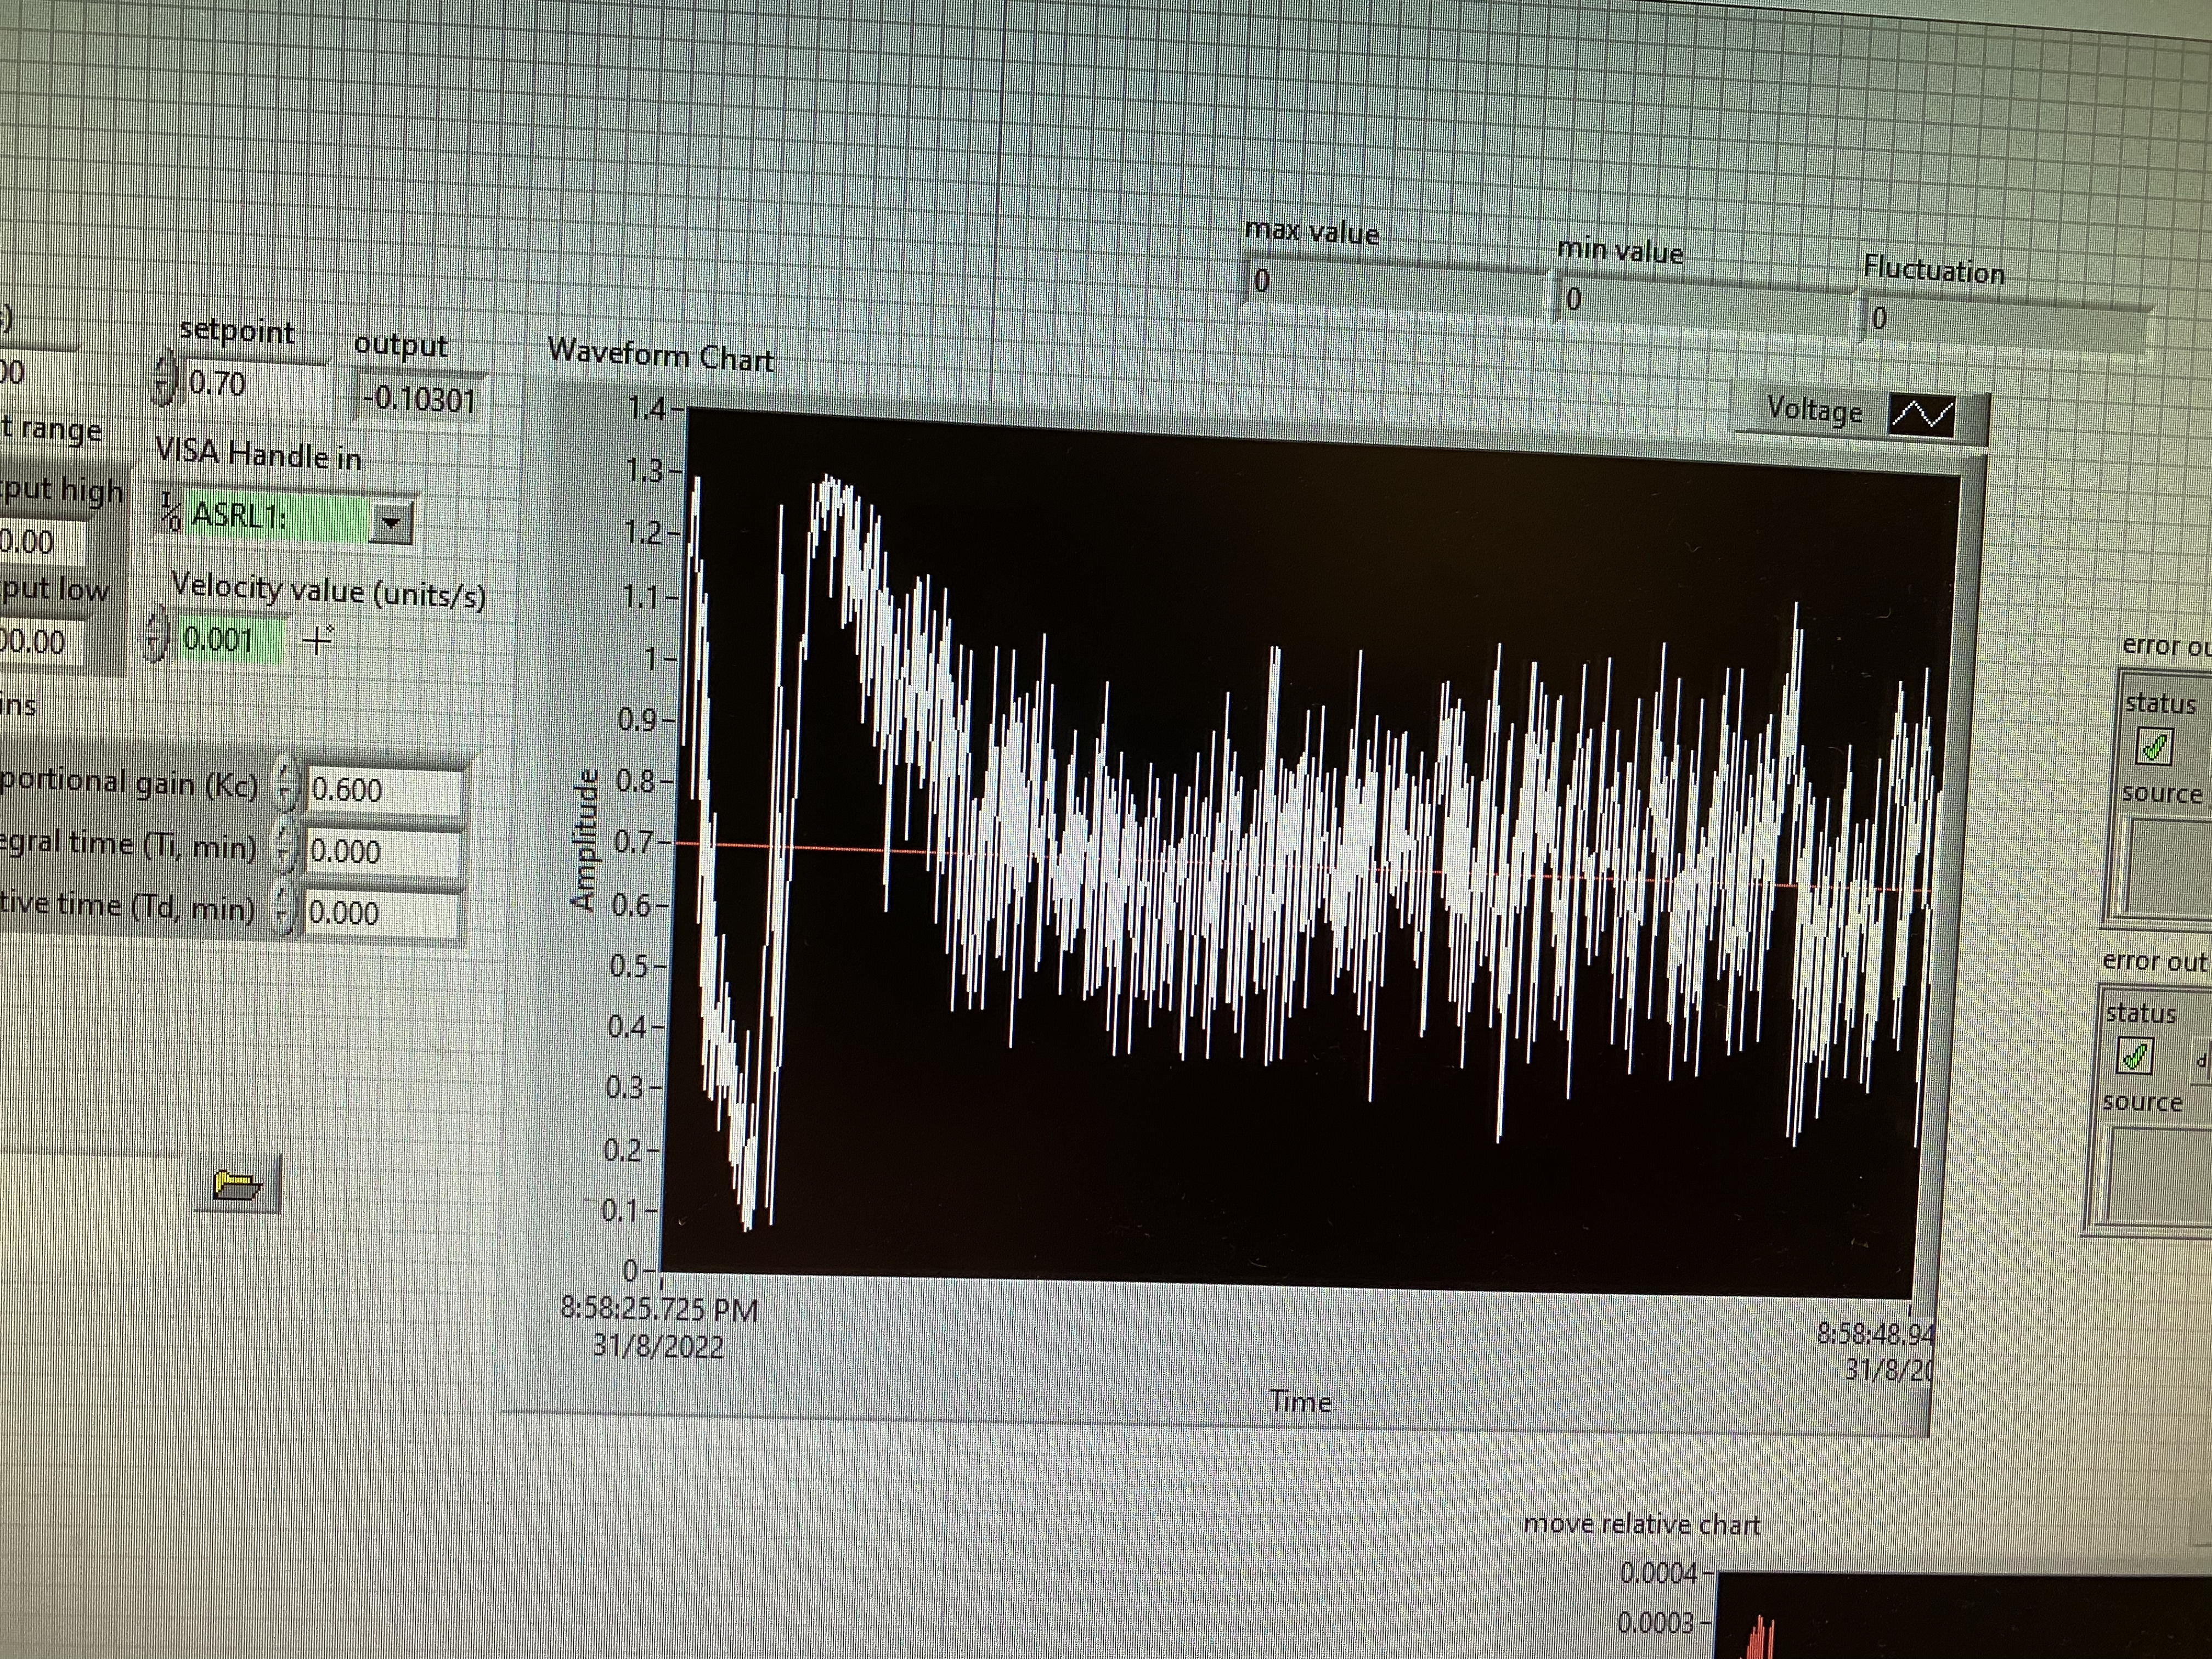
\includegraphics[width=0.4\textwidth,angle=0,origin=c]{pictures/IMG_1349.jpg}
\end{figure}

\subsection{Here are some of the difficulties we faced:}



\subsubsection{The responsiveness of the motor}

The motor we used was the Newport SMC100 motor. It turns out that this motor is not responsive enough (small time delay in communication) and it makes the PID algorithm much worse than we expected. However, we have tried using a Picomotor from Newport as well, which could move in a much smaller scale , with higher precision. After testing, we found out there is instability issue of the motor. It shakes greatly occasionally and caused failure of PID.

\subsubsection{TThe PID algorithm might not be the appropriate algorithm}

The PID algorithm responds proportionally to the error, ie, the output is larger when setpoint - input is larger. In this interference controller, the output is positive when the error is positive, and positive output refers to motor moving forward. The problem is that the moving the motor forward doesn’t necessarily increase the intensity of the inference. The plotting of Intensity against displacement of motor is Sine Curve- like , but shifted upwards. And as we know, moving forward from 0 degree of the curve increases the intensity, while moving forward from 90 degree decreases the intensity. This is a major reason I think the PID algorithm might not be an appropriate algorithm in this scenario.



\section{Interference Lithography}

The last thing I have learnt in this research intern is Interference Lithography. It is a method to build gratings onto silicon wafers. It is a fantastic experience because Interference Lithography is used while making Computer Processors (MOSFET). As an Electrical and Electronic Engineering student, I am allowed to dive deeper this field.

Reference:
The Entire World Relies on a Machine Made by ONE Company
ASML is a company that produces machines to make computer chips, and they use lithography (with light of different frequency). The gernal concept is the same as we used.

\begin{figure}[H]
\centering
\includegraphics[width=0.3\textwidth,angle=0,origin=c]{pictures/lithographymosfet.png}
\end{figure}


The photoresist we used is AZ 5214 E Photoresist. More info and data can be referred at:


\url{https://www.microchemicals.com/products/photoresists/az\_5214\_e.html}
\\
\url{https://www.microchemicals.com/micro/tds\_az\_5214e\_photoresist.pdf}

\subsection{Preparation:}

To perform Interference Lithography, silicon wafers are used. Everything should be clean to perform the lithography as small impurities/dusts can impact the result adversely. So before starting the process, clean the wafers with cotton buds soaked in ethanol to clear the Dust.


\begin{figure}[H]
\centering
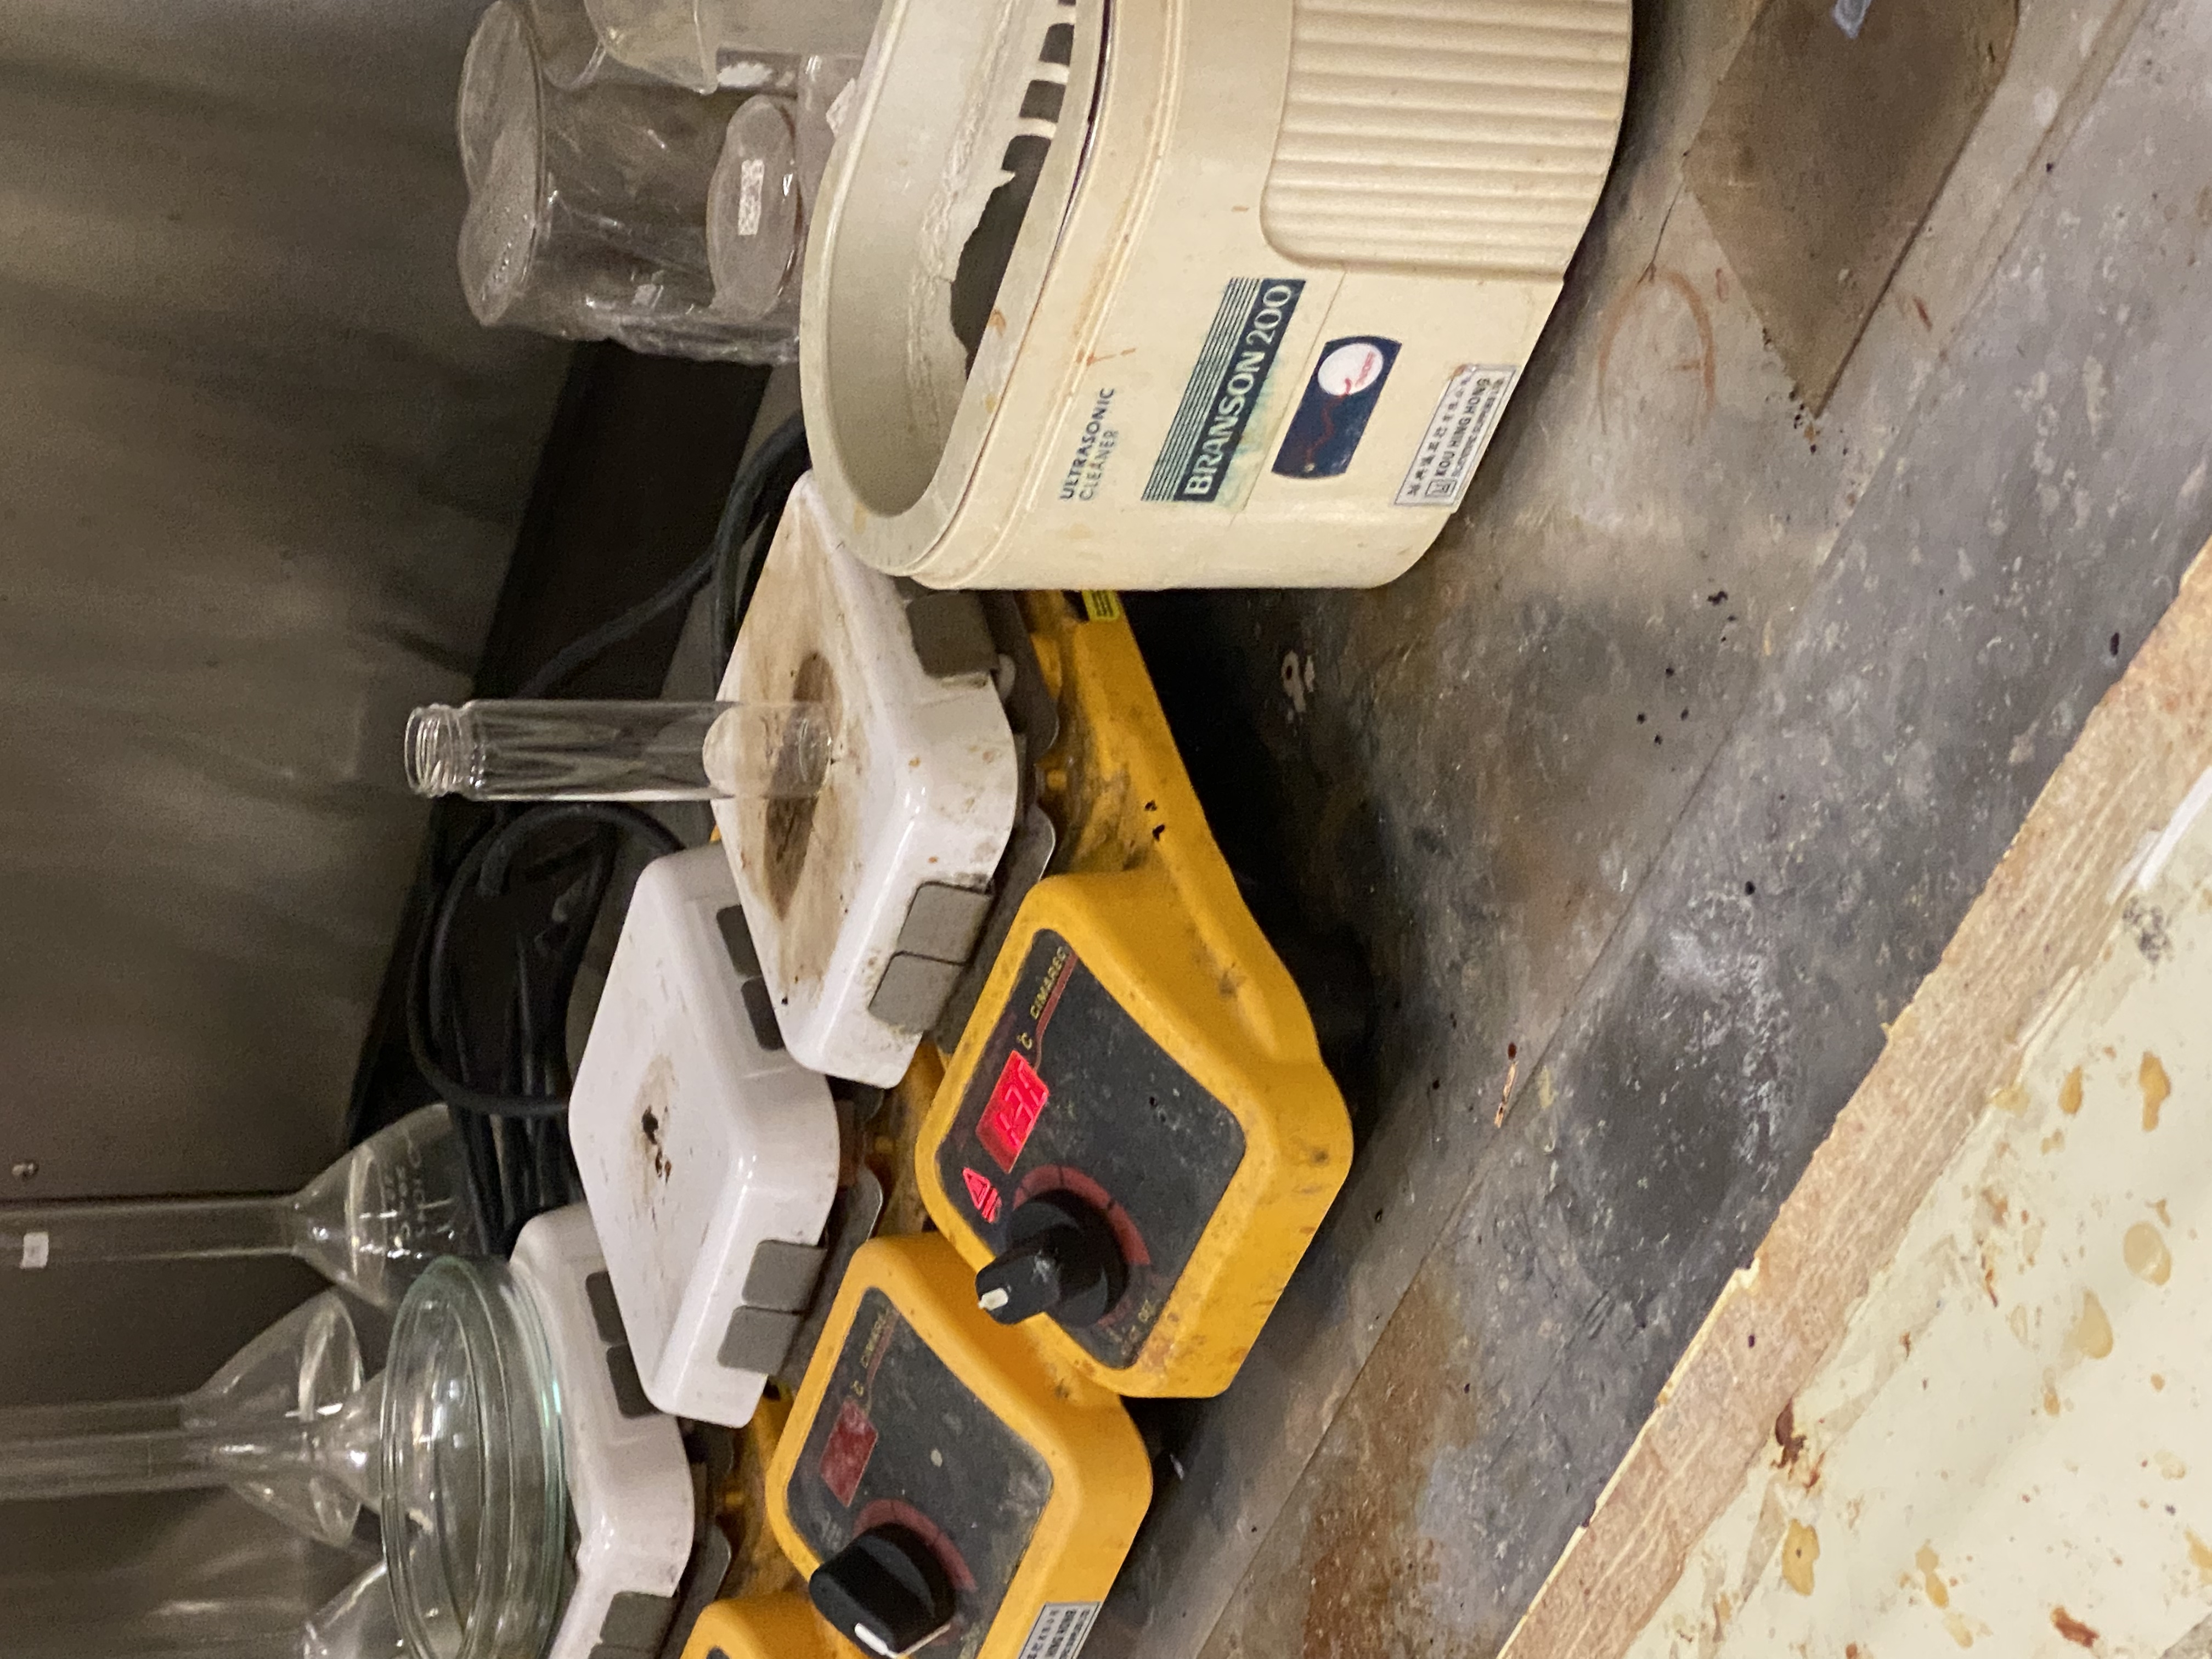
\includegraphics[width=0.4\textwidth,angle=-90,origin=c]{pictures/IMG_1581.jpg}
\end{figure}


\subsection{reparing photoresist:}

The photoresist we used is AZ 5214 E and in order to produce gratings with different thicknesses, different concentrations of photoresists are used. We choose to dilute the photoresist with 1:2 ratio mixing with solvent, after series of testing.


\subsection{Sample Cleaning:}

To remove ethanol and some other impurities, prebake the wafers at  250°C for 10 minutes.



\subsection{Spin Coating and Prebake:}

Pour about 50 uL of photoresist onto the wafer, and activate the spinner to perform spin coating for 1 minute. Then put the wafer onto the 110°C heater for 15 seconds.

\begin{figure}[H]
\centering
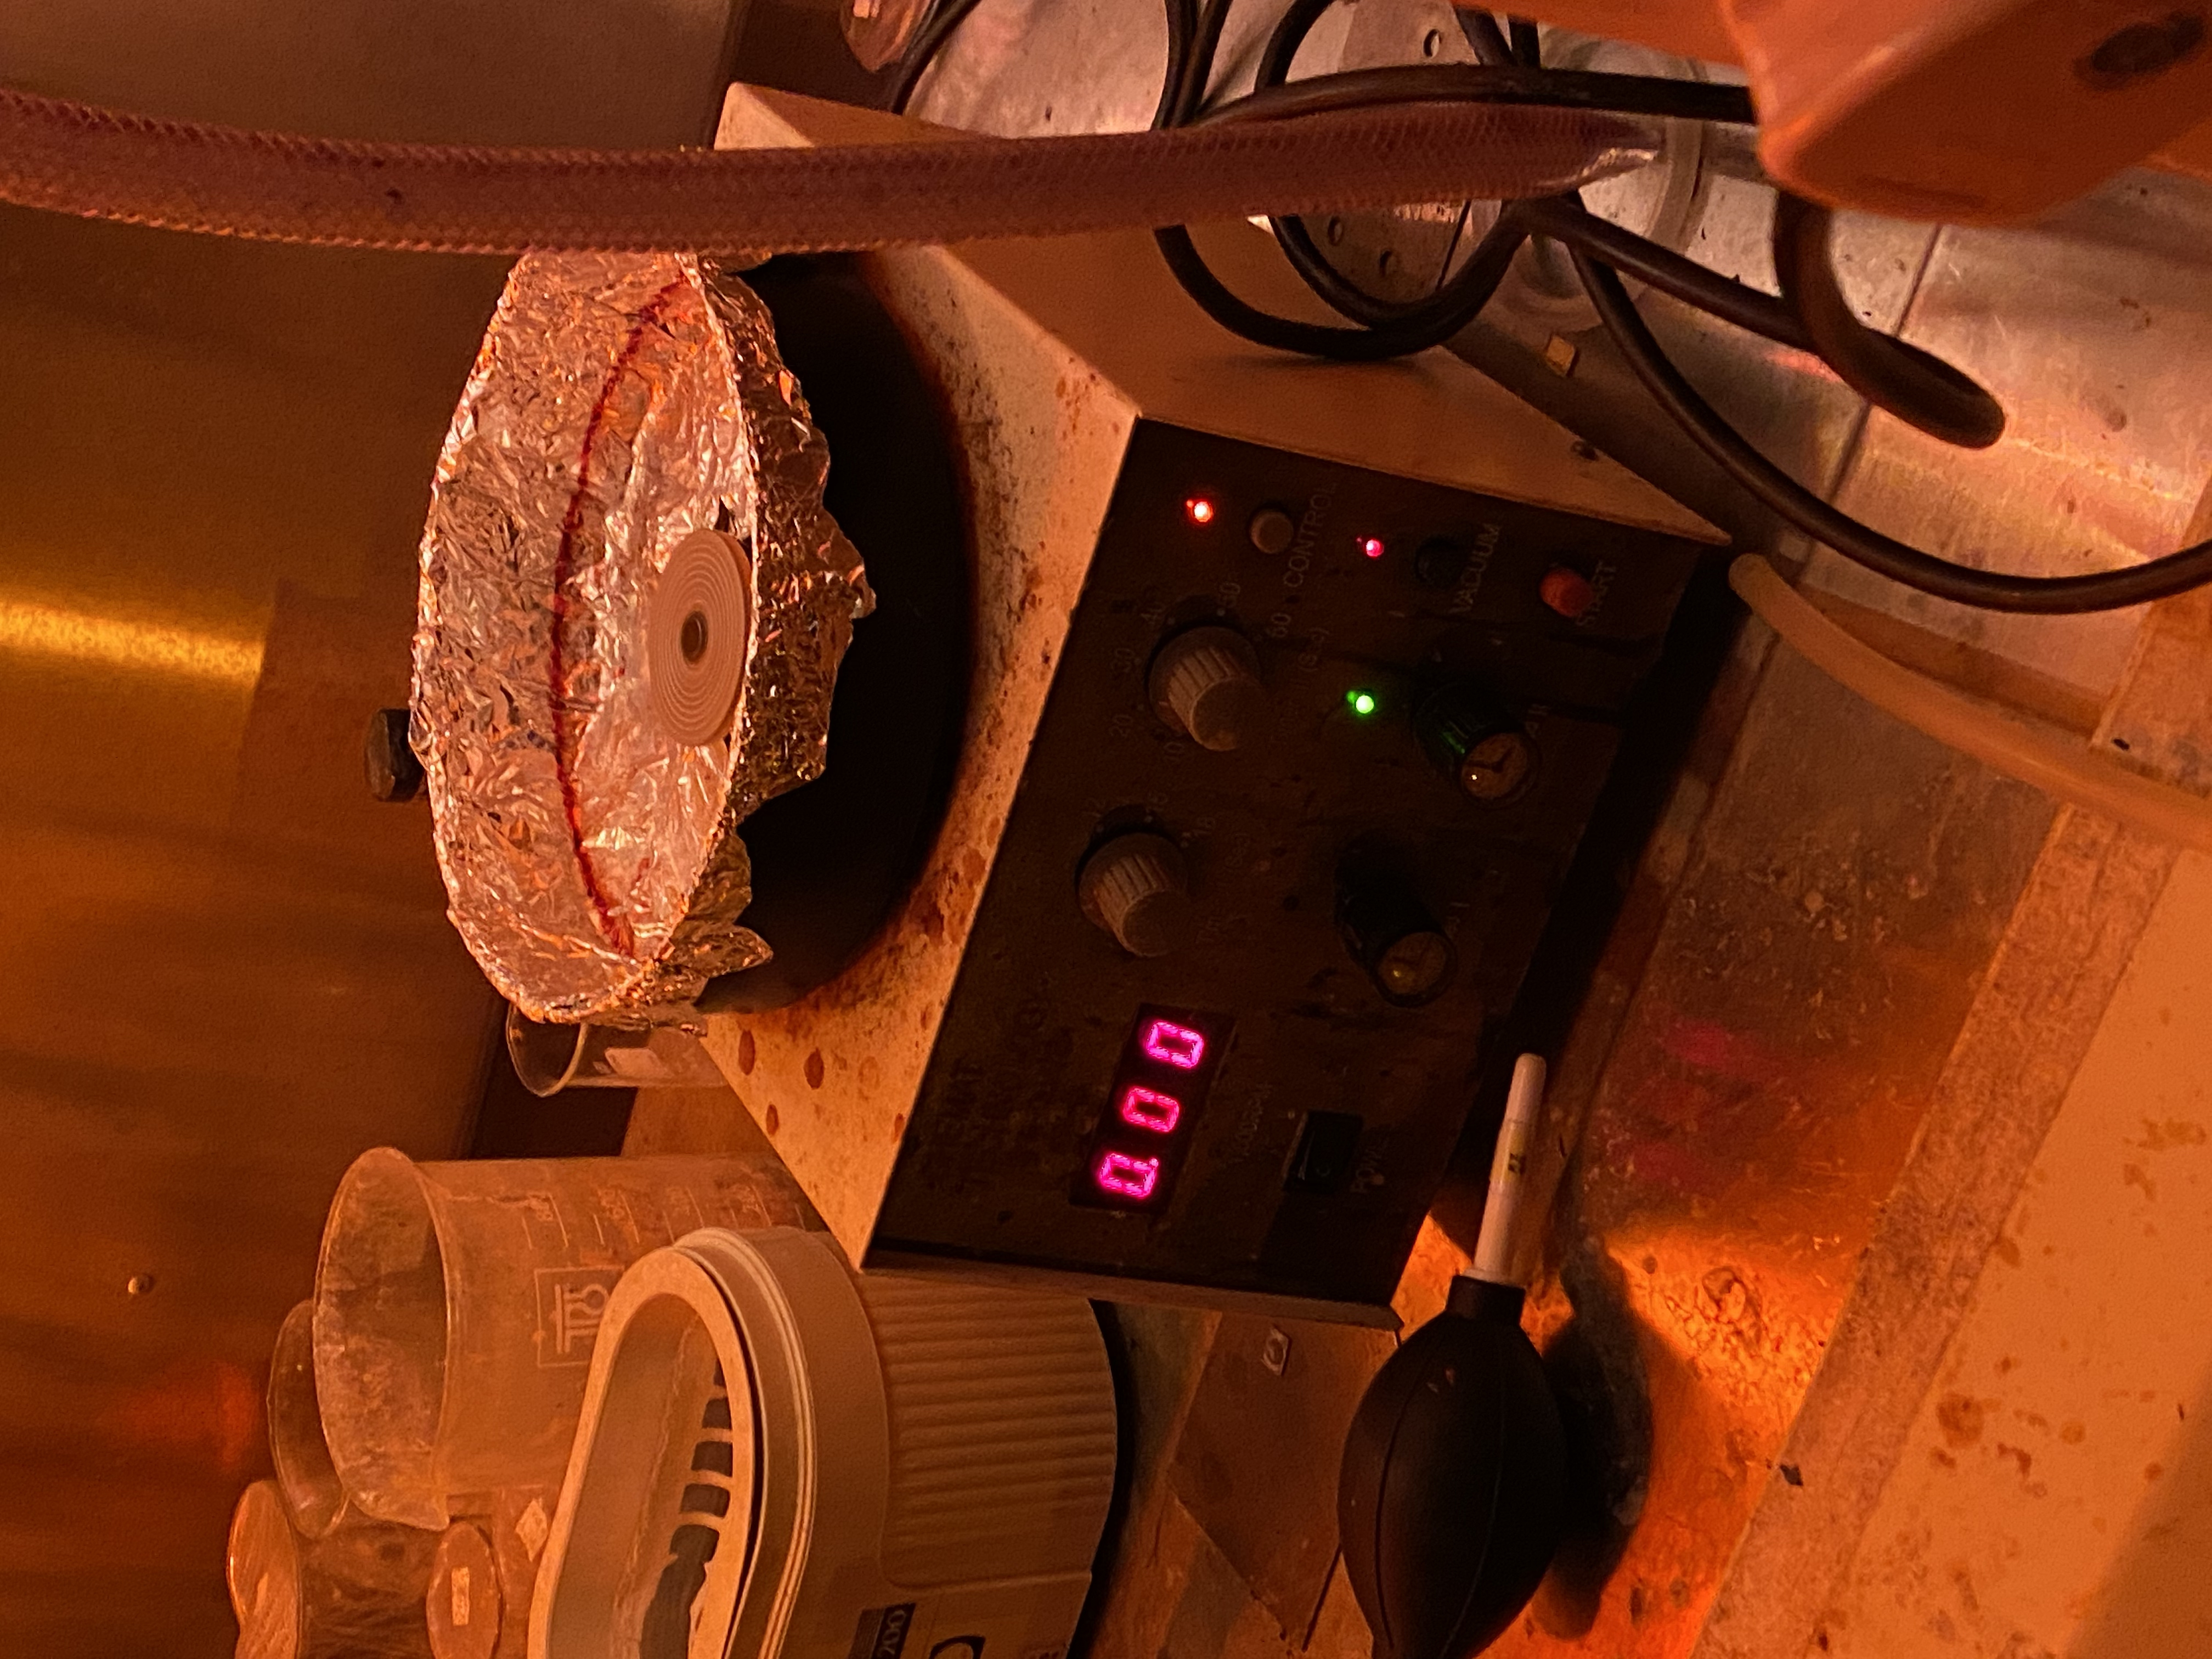
\includegraphics[width=0.4\textwidth,angle=-90,origin=c]{pictures/IMG_1584.jpg}
\end{figure}


\subsection{Exposure:}

Using the stable UV laser interference controlled by the PID algorithm we built, we shine the UV light onto the wafer for 4 minutes. Whole process is done without external light source with wavelength shorter than red light.

\subsection{The set-up used for exposure:}

\begin{figure}[H]
\centering
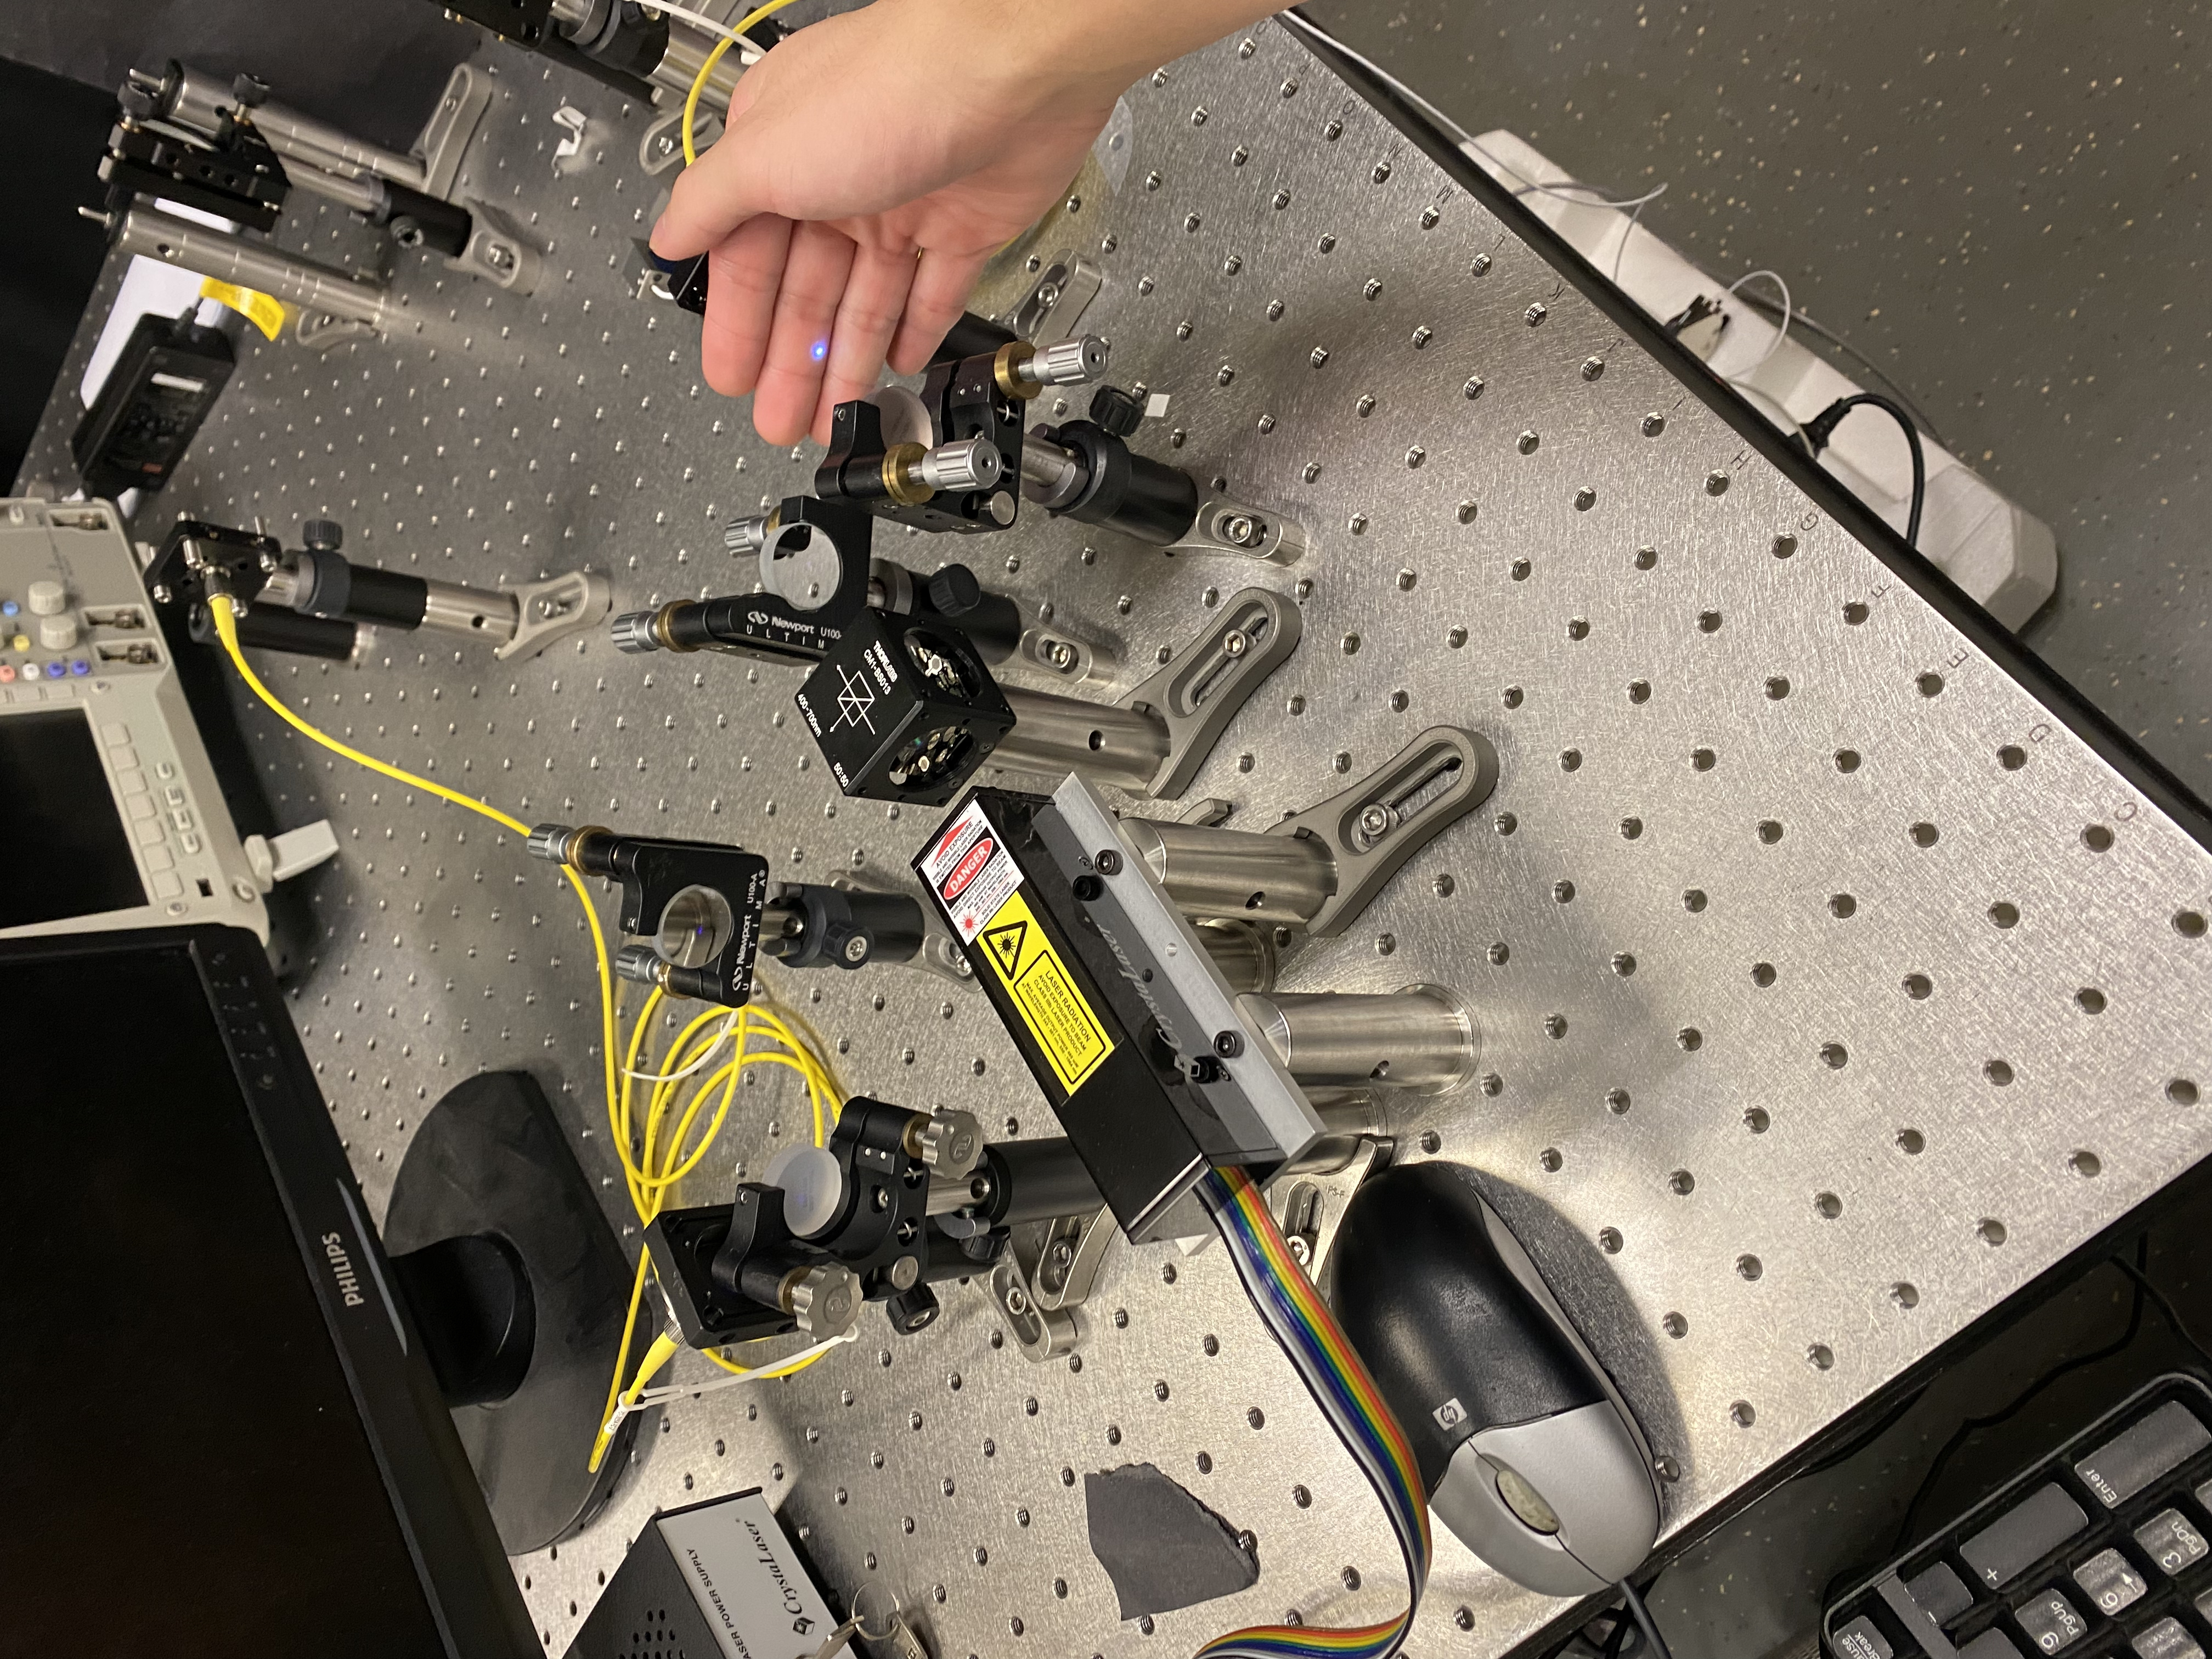
\includegraphics[width=0.4\textwidth,angle=-90,origin=c]{pictures/IMG_1736.jpg}
\end{figure}




\subsection{Reversal Bake and Development:}

Bake the wafers for 2 minutes at 120°C , then develop the sample using AZ 726 puddle. Then the gratings should be built.


\subsection{Reviewing the quality of sample under SEM (Scanning Electron Microscope):}

We can use SEM to determine the thickness of our gratings. We aimed to have a thickness of about 200 nanometres. We were able to achieve this after testing with different concentrations, spin RPM and development time/postbake time.

\subsubsection{Using of Scanning Electron Microscope:}

\begin{figure}[H]
\centering
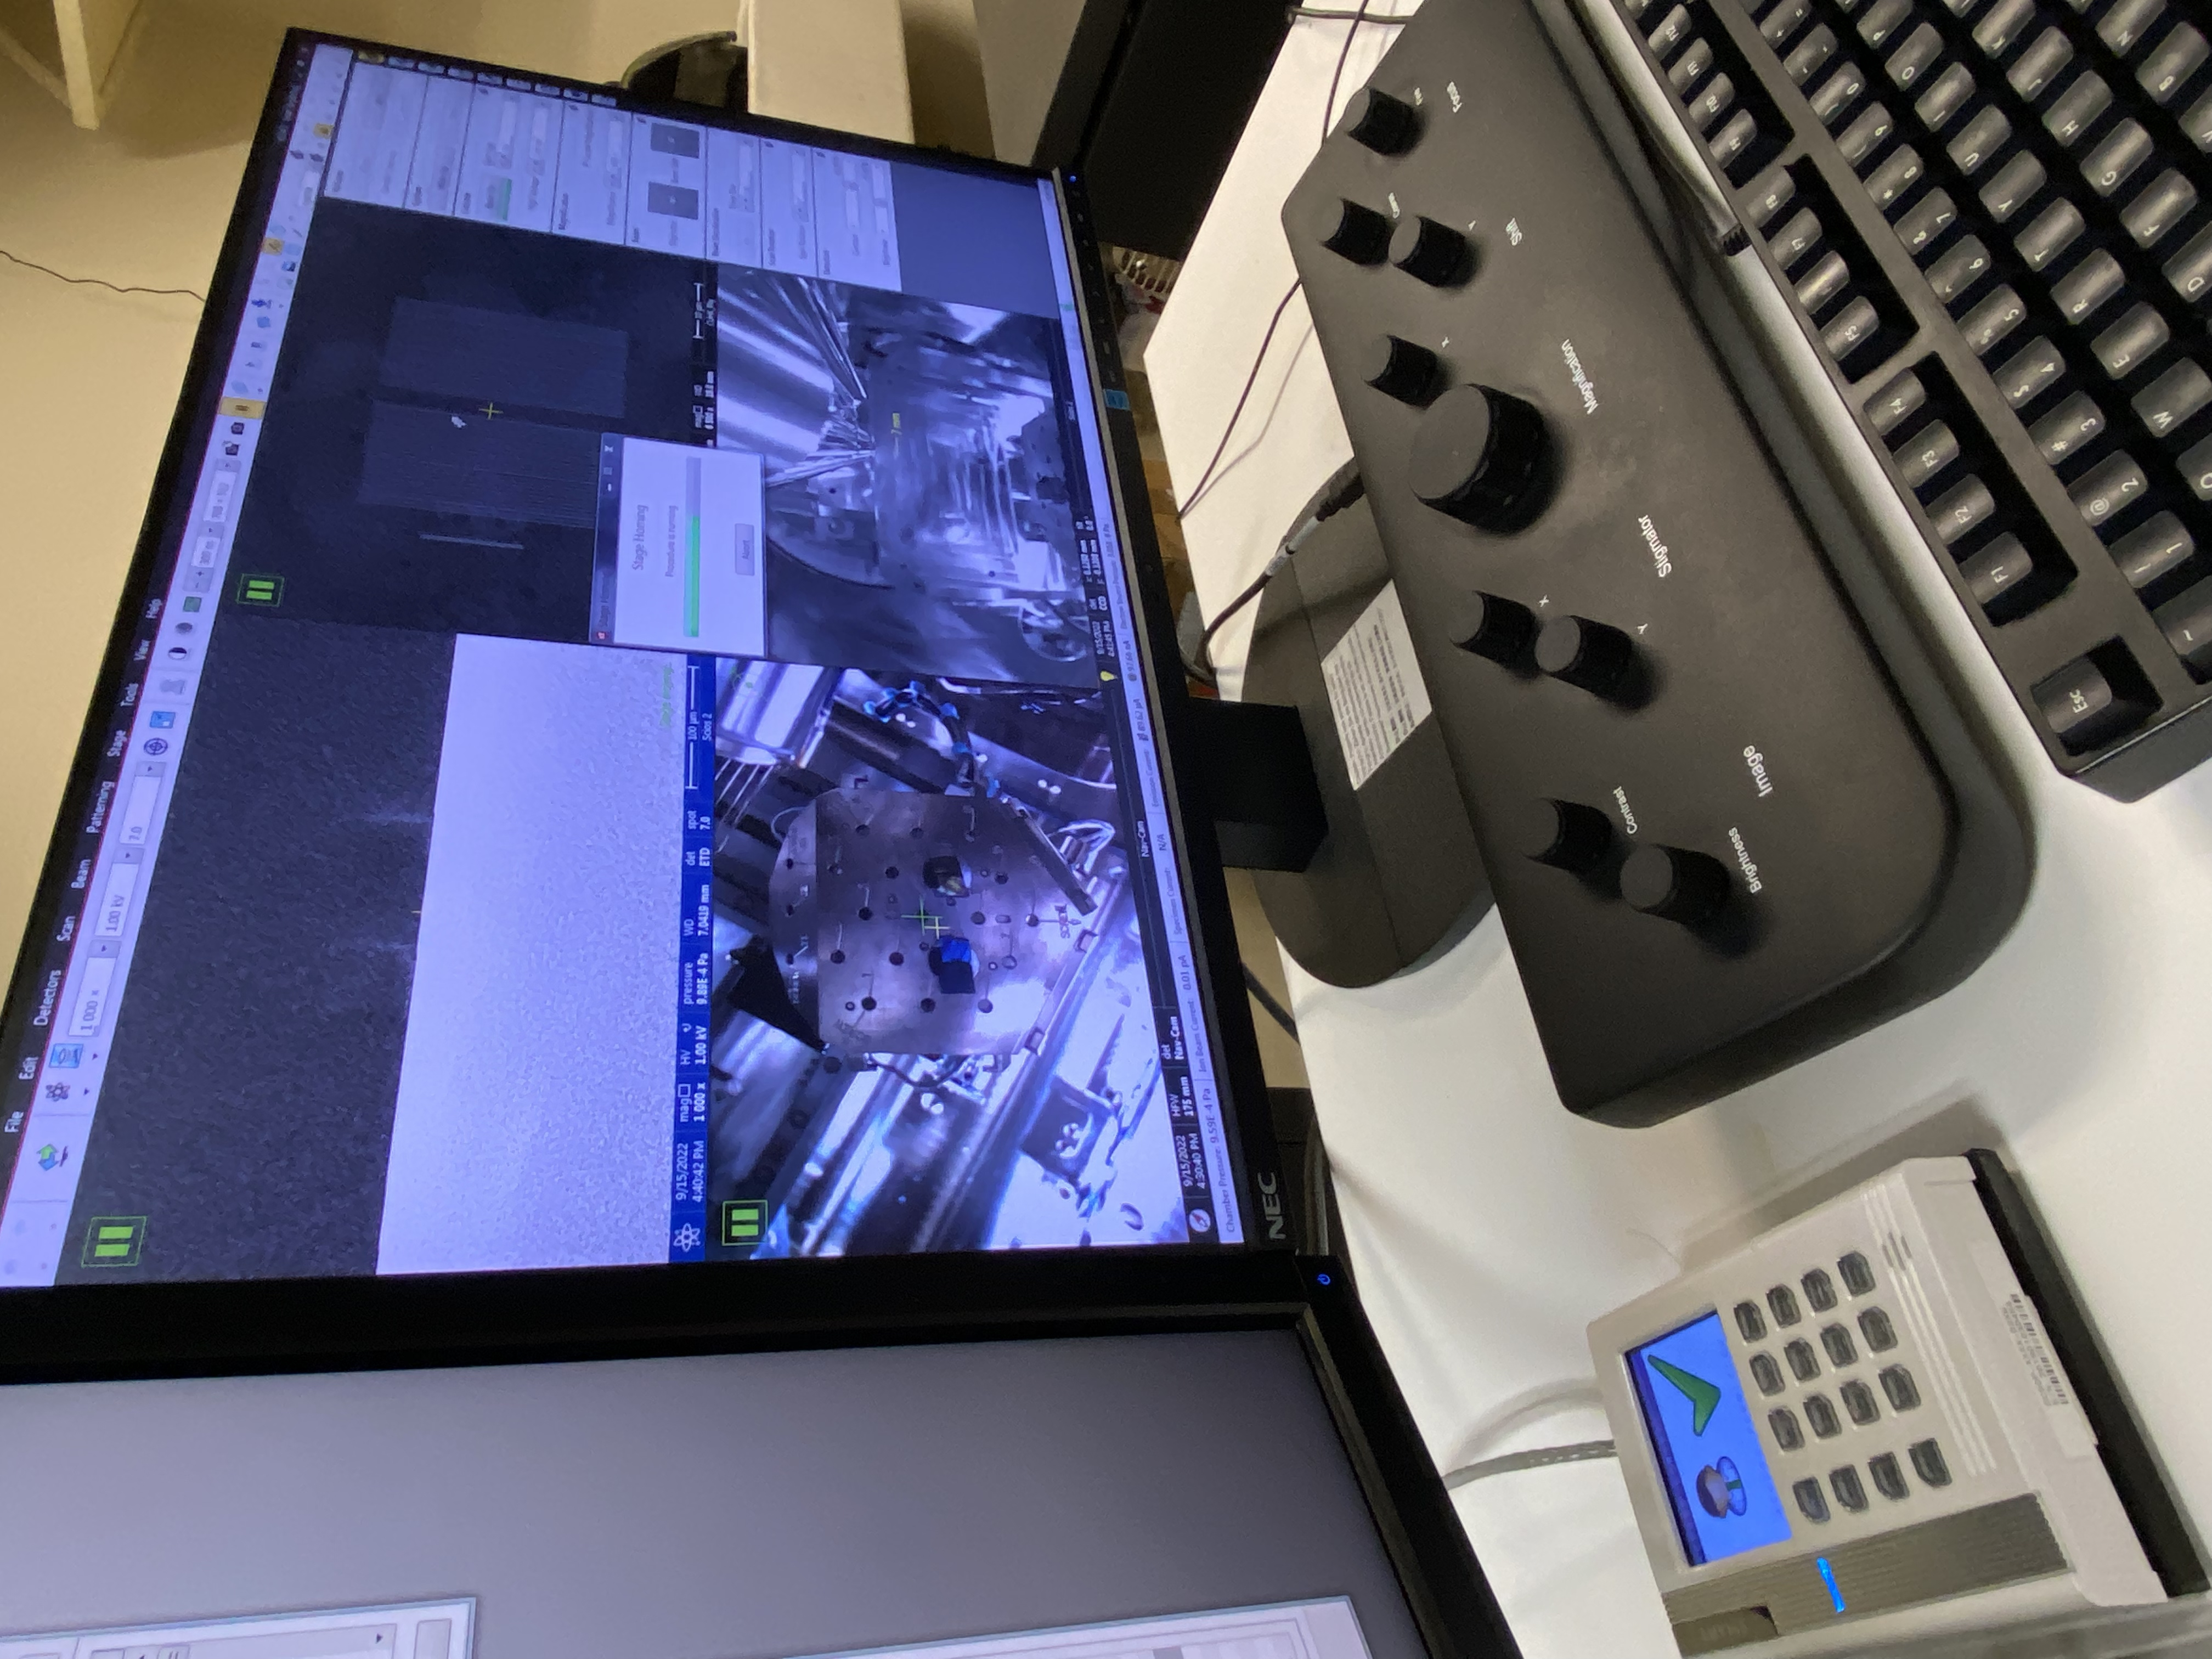
\includegraphics[width=0.3\textwidth,angle=-90,origin=c]{pictures/IMG_1586.jpg}

\includegraphics[width=0.3\textwidth,angle=0,origin=c]{pictures/IMG_1585.jpg}

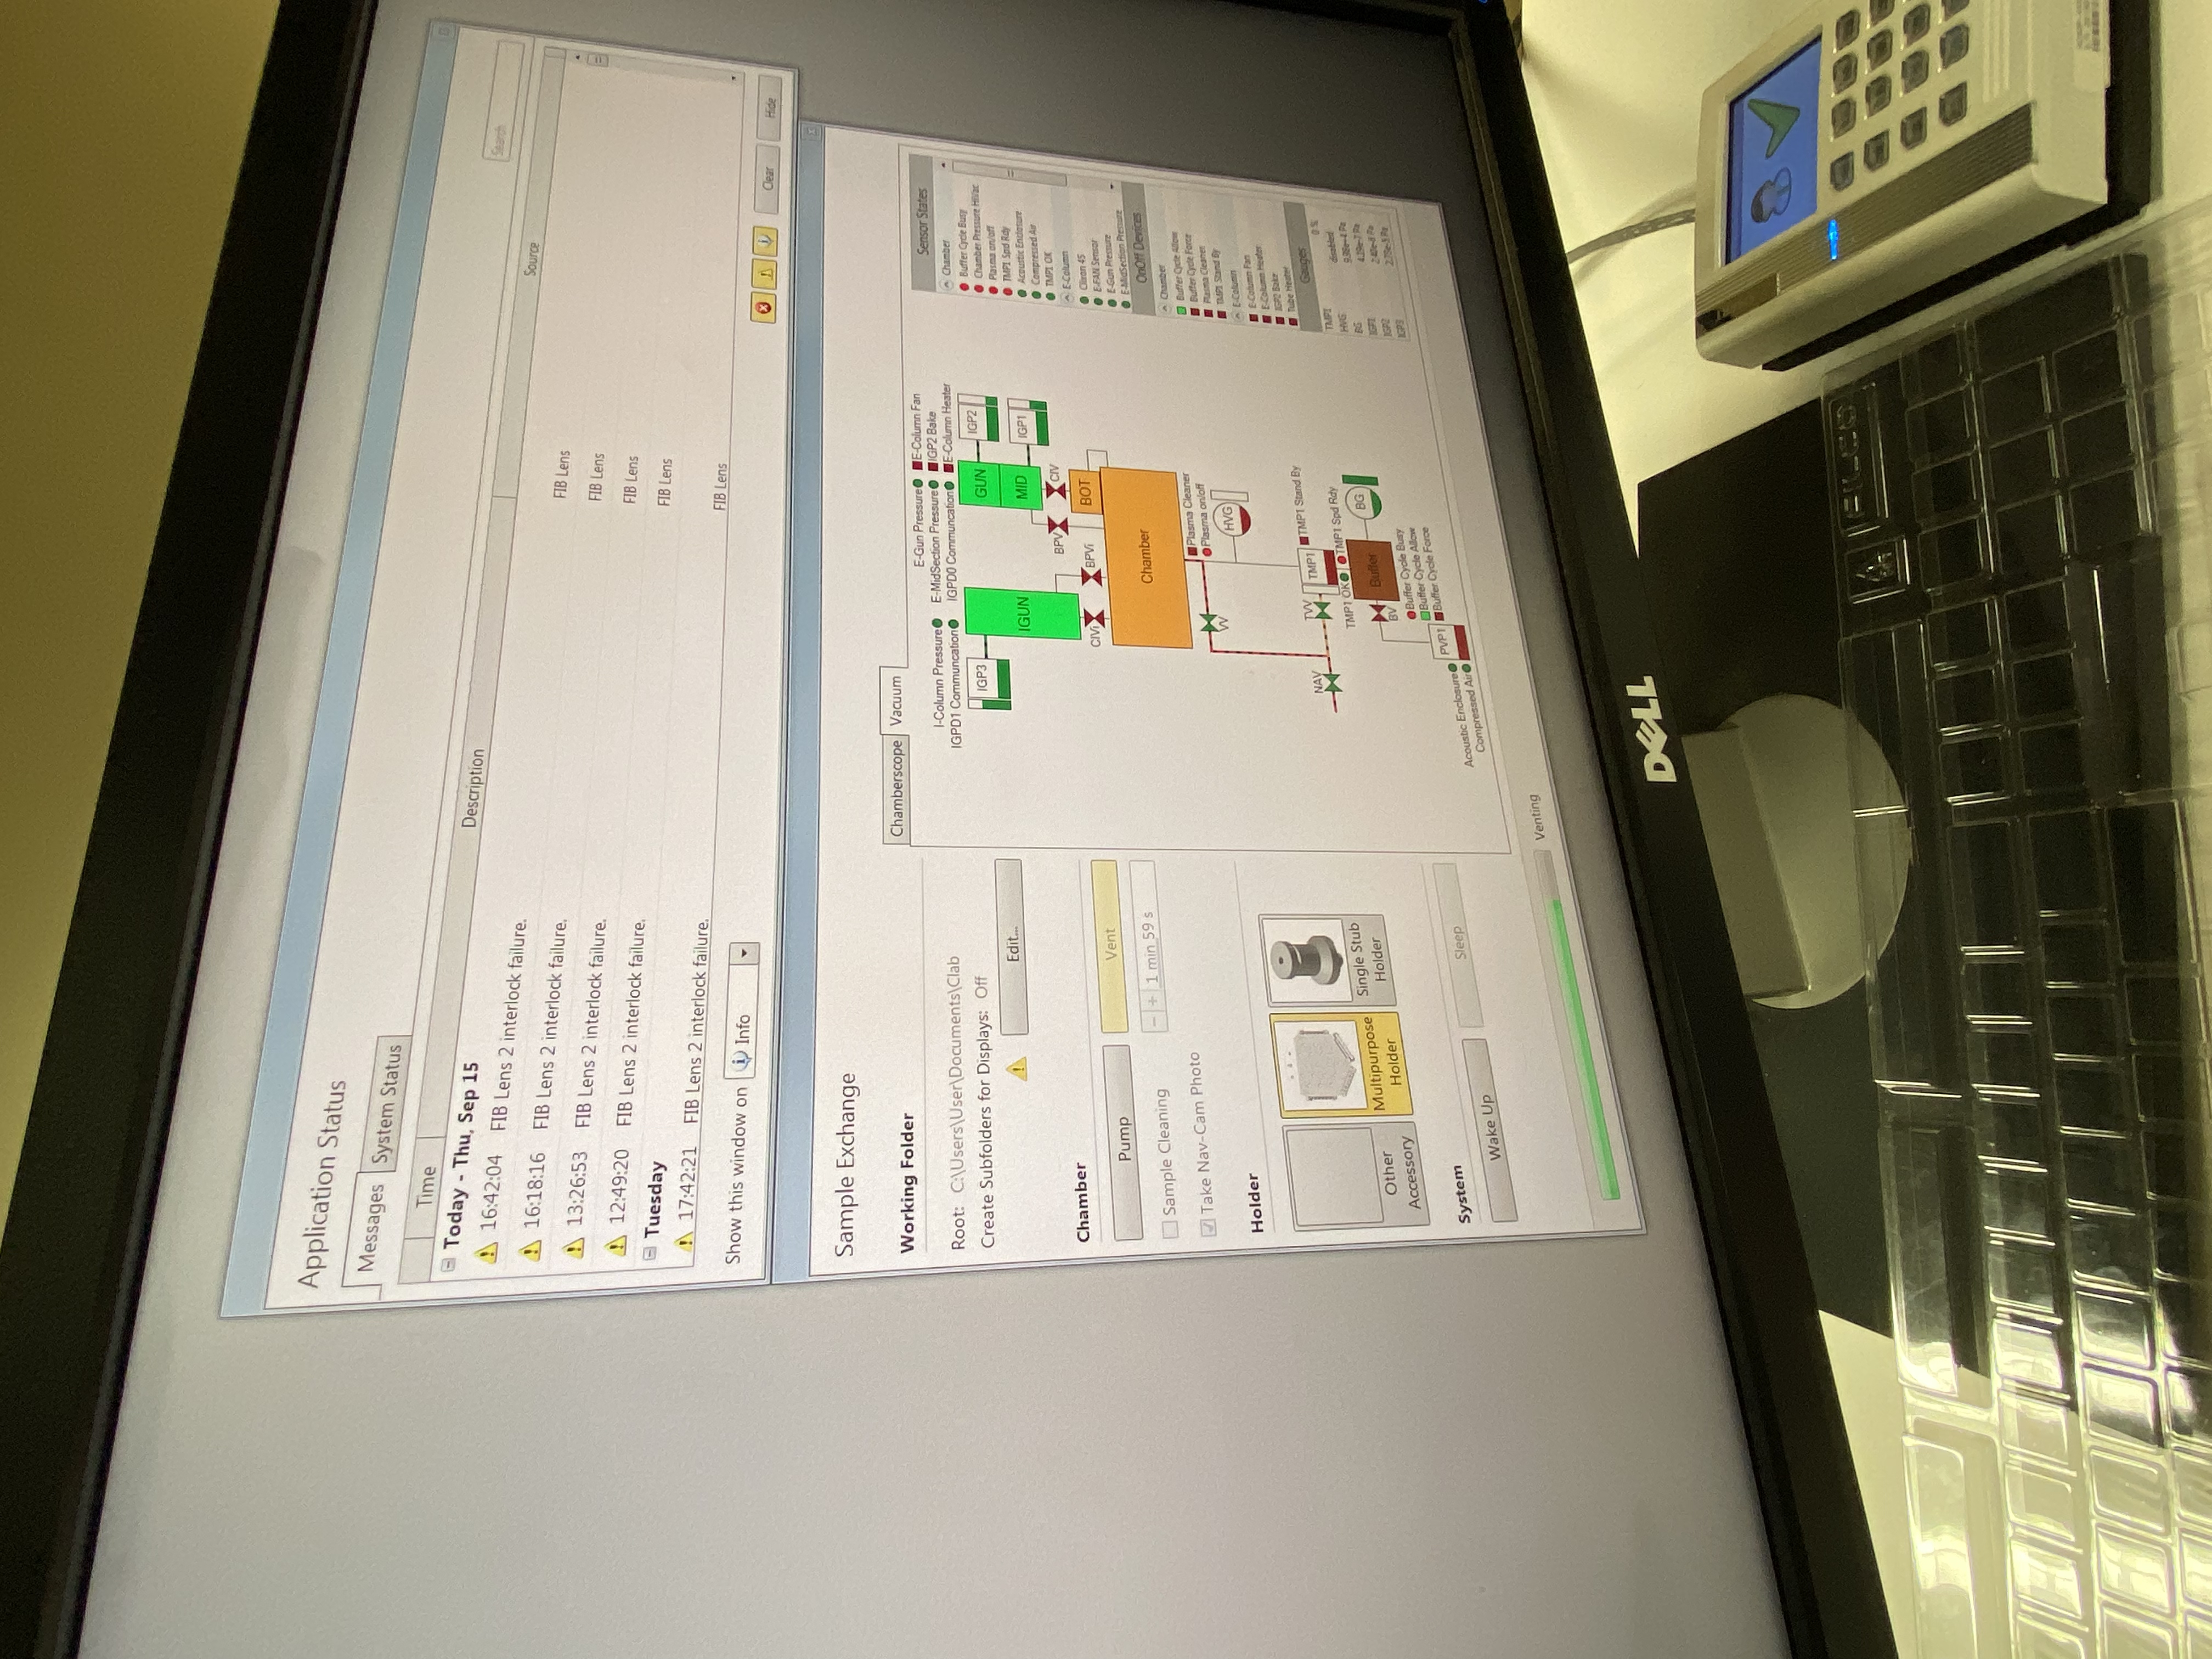
\includegraphics[width=0.3\textwidth,angle=-90,origin=c]{pictures/IMG_1588.jpg}

\end{figure}



\section{Conclusion:}

It was an amazing internship experience as I have learnt much more in the field of software engineering and physics. I started from zero as I did not have any knowledge in Michelson Interferometer, PID and even Lithography. I learnt relevant knowledge through the internship. I believe this experience has built me a basis to get into the relevant industries.
\end{document}


